\documentclass[8pt]{article}
\usepackage[]{algorithm2e}
\usepackage{subcaption}
\usepackage{pbox}
\usepackage{balance}
\usepackage{graphicx}
\usepackage[a4paper,  margin=1cm]{geometry}

\title{Reproducing computational results of: ``Follow the Leader: Alternating CPU/GPU Computations in PDES''}

\author{}
\date{}
\begin{document}

\maketitle

\section*{Hardware/software configuration}
{\scriptsize
\begin{minipage}[t]{0.45\textwidth}
Authors' configuration:
\begin{itemize}
\item CPU: AMD Ryzen 9 7950x
\item GPU: NVIDIA RTX 3090 Ti
\item RAM: 64GB
\end{itemize}
\end{minipage}
\begin{minipage}[t]{0.45\textwidth}
RCR:
\begin{itemize}
\input{run_logs/machine.tex}
\end{itemize}
\end{minipage}
}
\setcounter{figure}{2}

\section*{Figure 2}

\newcommand{\mysize}{0.75\linewidth}


\renewcommand{\mysize}{0.45\linewidth}

\setcounter{figure}{1}
\renewcommand{\thefigure}{\arabic{figure}a}
\begin{figure}[!h]
\centering
\begin{subfigure}[b]{\mysize}
\centering
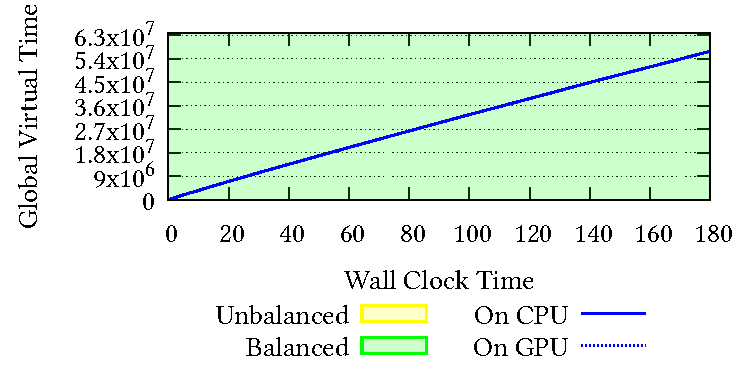
\includegraphics[width=0.8\textwidth]{figures_original/balanced/1.processed.pdf}
\renewcommand{\thesubfigure}{Original}
\caption{}
\end{subfigure}
\begin{subfigure}[b]{\mysize}
\centering
\IfFileExists{run_logs/balanced/1.processed.pdf}{
\includegraphics[width=0.8\textwidth]{run_logs/balanced/1.processed.pdf}
}{\texttt{run\_logs/balanced/1.processed.pdf} not found, please run \texttt{./exp.sh run\_balanced} first}
\renewcommand{\thesubfigure}{Reproduced}
\caption{}
\end{subfigure}
\caption{CPU only – Balanced}
\end{figure}


\setcounter{figure}{1}
\renewcommand{\thefigure}{\arabic{figure}d}
\begin{figure}[!h]
\centering
\begin{subfigure}[b]{\mysize}
\centering
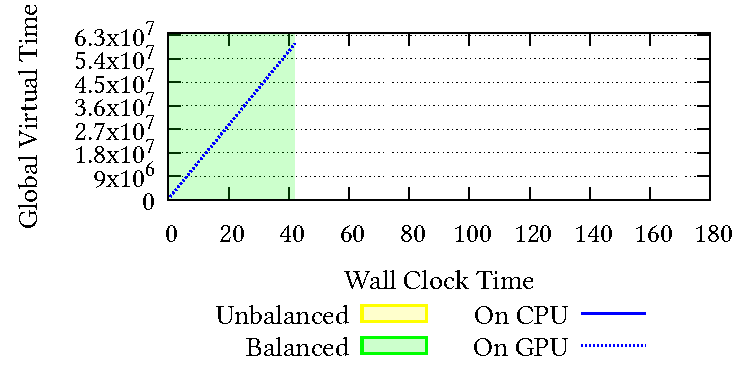
\includegraphics[width=0.8\textwidth]{figures_original/balanced/2.processed.pdf}
\renewcommand{\thesubfigure}{Original}
\caption{}
\end{subfigure}
\begin{subfigure}[b]{\mysize}
\centering
\IfFileExists{run_logs/balanced/2.processed.pdf}{
\includegraphics[width=0.8\textwidth]{run_logs/balanced/2.processed.pdf}
}{\texttt{run\_logs/balanced/2.processed.pdf} not found, please run \texttt{./exp.sh run\_all} first}
\renewcommand{\thesubfigure}{Reproduced}
\caption{}
\end{subfigure}
\caption{GPU only – Balanced}
\end{figure}



\setcounter{figure}{1}
\renewcommand{\thefigure}{\arabic{figure}g}
\begin{figure}[!h]
\centering
\begin{subfigure}[b]{\mysize}
\centering
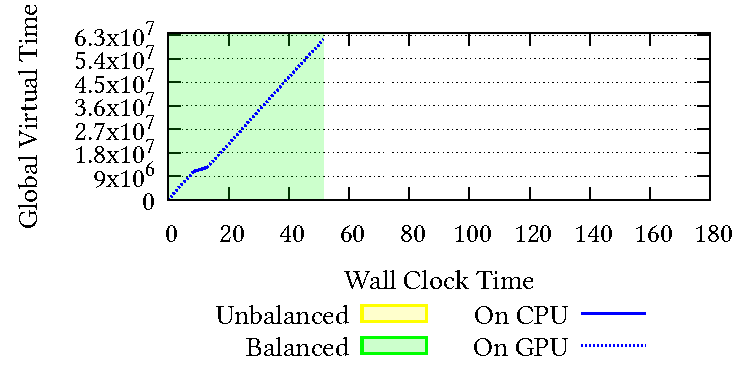
\includegraphics[width=0.8\textwidth]{figures_original/balanced/3.processed.pdf}
\renewcommand{\thesubfigure}{Original}
\caption{}
\end{subfigure}
\begin{subfigure}[b]{\mysize}
\centering
\IfFileExists{run_logs/balanced/3.processed.pdf}{
\includegraphics[width=0.8\textwidth]{run_logs/balanced/3.processed.pdf}
}{\texttt{run\_logs/balanced/3.processed.pdf} not found, please run \texttt{./exp.sh run\_all} first}
\renewcommand{\thesubfigure}{Reproduced}
\caption{}
\end{subfigure}
\caption{Follow the leader – Balanced}
\end{figure}



%####################################################################################################
%####################################################################################################
%####################################################################################################
%####################################################################################################
%####################################################################################################

\clearpage


\setcounter{figure}{1}
\renewcommand{\thefigure}{\arabic{figure}b}
\begin{figure}[!h]
\centering
\begin{subfigure}[b]{\mysize}
\centering
\includegraphics[width=0.8\textwidth]{figures_original/unbalanced/1.processed.pdf}
\renewcommand{\thesubfigure}{Original}
\caption{}
\end{subfigure}
\begin{subfigure}[b]{\mysize}
\centering
\IfFileExists{run_logs/unbalanced/1.processed.pdf}{
\includegraphics[width=0.8\textwidth]{run_logs/unbalanced/1.processed.pdf}
}{\texttt{run\_logs/unbalanced/1.processed.pdf} not found, please run \texttt{./exp.sh run\_unbalanced} first}
\renewcommand{\thesubfigure}{Reproduced}
\caption{}
\end{subfigure}
\caption{CPU only – Unbalanced}
\end{figure}


\setcounter{figure}{1}
\renewcommand{\thefigure}{\arabic{figure}e}
\begin{figure}[!h]
\centering
\begin{subfigure}[b]{\mysize}
\centering
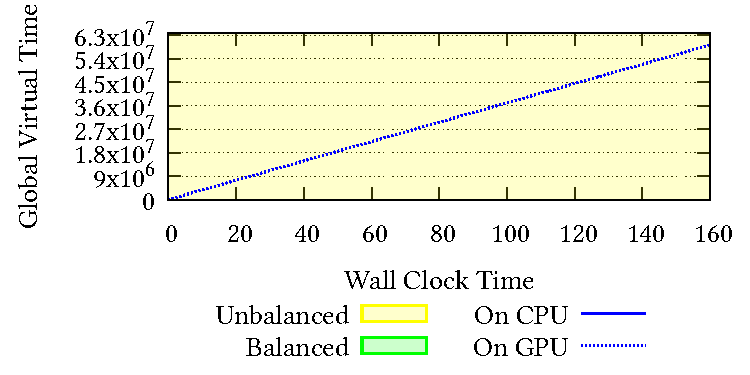
\includegraphics[width=0.8\textwidth]{figures_original/unbalanced/2.processed.pdf}
\renewcommand{\thesubfigure}{Original}
\caption{}
\end{subfigure}
\begin{subfigure}[b]{\mysize}
\centering
\IfFileExists{run_logs/unbalanced/2.processed.pdf}{
\includegraphics[width=0.8\textwidth]{run_logs/unbalanced/2.processed.pdf}
}{\texttt{run\_logs/unbalanced/2.processed.pdf} not found, please run \texttt{./exp.sh run\_all} first}
\renewcommand{\thesubfigure}{Reproduced}
\caption{}
\end{subfigure}
\caption{GPU only – Unbalanced}
\end{figure}



\setcounter{figure}{1}
\renewcommand{\thefigure}{\arabic{figure}h}
\begin{figure}[!h]
\centering
\begin{subfigure}[b]{\mysize}
\centering
\includegraphics[width=0.8\textwidth]{figures_original/unbalanced/3.processed.pdf}
\renewcommand{\thesubfigure}{Original}
\caption{}
\end{subfigure}
\begin{subfigure}[b]{\mysize}
\centering
\IfFileExists{run_logs/unbalanced/3.processed.pdf}{
\includegraphics[width=0.8\textwidth]{run_logs/unbalanced/3.processed.pdf}
}{\texttt{run\_logs/unbalanced/3.processed.pdf} not found, please run \texttt{./exp.sh run\_all} first}
\renewcommand{\thesubfigure}{Reproduced}
\caption{}
\end{subfigure}
\caption{Follow the leader – Unbalanced}
\end{figure}





%####################################################################################################
%####################################################################################################
%####################################################################################################
%####################################################################################################
%####################################################################################################

\clearpage


\setcounter{figure}{1}
\renewcommand{\thefigure}{\arabic{figure}c}
\begin{figure}[!h]
\centering
\begin{subfigure}[b]{\mysize}
\centering
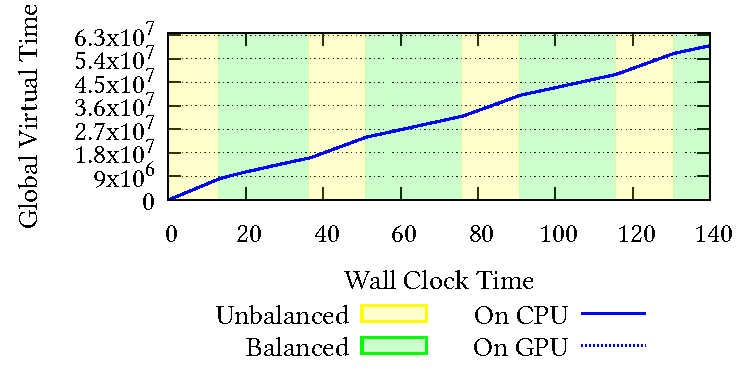
\includegraphics[width=0.8\textwidth]{figures_original/alternating/1.processed.pdf}
\renewcommand{\thesubfigure}{Original}
\caption{}
\end{subfigure}
\begin{subfigure}[b]{\mysize}
\centering
\IfFileExists{run_logs/alternating/1.processed.pdf}{
\includegraphics[width=0.8\textwidth]{run_logs/alternating/1.processed.pdf}
}{\texttt{run\_logs/alternating/1.processed.pdf} not found, please run \texttt{./exp.sh run\_alternating} first}
\renewcommand{\thesubfigure}{Reproduced}
\caption{}
\end{subfigure}
\caption{CPU only – Alternating Phases}
\end{figure}


\setcounter{figure}{1}
\renewcommand{\thefigure}{\arabic{figure}f}
\begin{figure}[!h]
\centering
\begin{subfigure}[b]{\mysize}
\centering
\includegraphics[width=0.8\textwidth]{figures_original/alternating/2.processed.pdf}
\renewcommand{\thesubfigure}{Original}
\caption{}
\end{subfigure}
\begin{subfigure}[b]{\mysize}
\centering
\IfFileExists{run_logs/alternating/2.processed.pdf}{
\includegraphics[width=0.8\textwidth]{run_logs/alternating/2.processed.pdf}
}{\texttt{run\_logs/alternating/2.processed.pdf} not found, please run \texttt{./exp.sh run\_all} first}
\renewcommand{\thesubfigure}{Reproduced}
\caption{}
\end{subfigure}
\caption{GPU only – Alternating Phases}
\end{figure}



\setcounter{figure}{1}
\renewcommand{\thefigure}{\arabic{figure}i}
\begin{figure}[!h]
\centering
\begin{subfigure}[b]{\mysize}
\centering
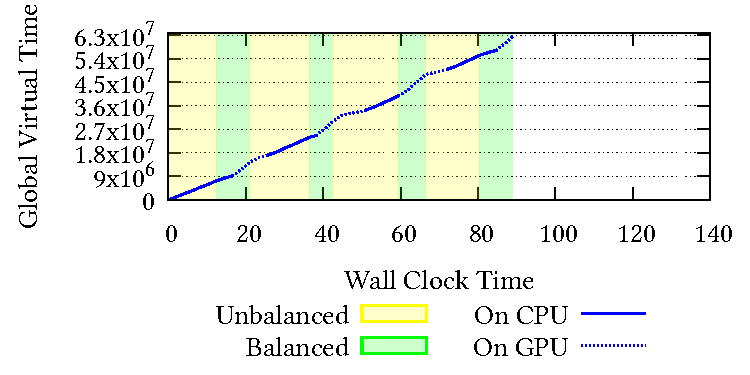
\includegraphics[width=0.8\textwidth]{figures_original/alternating/3.processed.pdf}
\renewcommand{\thesubfigure}{Original}
\caption{}
\end{subfigure}
\begin{subfigure}[b]{\mysize}
\centering
\IfFileExists{run_logs/alternating/3.processed.pdf}{
\includegraphics[width=0.8\textwidth]{run_logs/alternating/3.processed.pdf}
}{\texttt{run\_logs/alternating/3.processed.pdf} not found, please run \texttt{./exp.sh run\_all} first}
\renewcommand{\thesubfigure}{Reproduced}
\caption{}
\end{subfigure}
\caption{Follow the leader – Alternating Phases}
\end{figure}




%####################################################################################################
%####################################################################################################
% FIGURE 3
%####################################################################################################
%####################################################################################################


\clearpage

\section*{Figure 3}


\setcounter{figure}{2}
\renewcommand{\thefigure}{\arabic{figure}a}
\begin{figure}[!h]
\centering
\begin{subfigure}[b]{\mysize}
\centering
\includegraphics[width=0.8\textwidth]{figures_original/balanced.energy.pdf}
\renewcommand{\thesubfigure}{Original}
\caption{}
\end{subfigure}
\begin{subfigure}[b]{\mysize}
\centering
\IfFileExists{run_logs/balanced.energy.pdf}{
\includegraphics[width=0.8\textwidth]{run_logs/balanced.energy.pdf}
}{\texttt{run\_logs/balanced.energy.pdf} not found, please run \texttt{./exp.sh run\_alternating} first}
\renewcommand{\thesubfigure}{Reproduced}
\caption{}
\end{subfigure}
\caption{Balanced}
\end{figure}


\setcounter{figure}{1}
\renewcommand{\thefigure}{\arabic{figure}b}
\begin{figure}[!h]
\centering
\begin{subfigure}[b]{\mysize}
\centering
\includegraphics[width=0.8\textwidth]{figures_original/unbalanced.energy.pdf}
\renewcommand{\thesubfigure}{Original}
\caption{}
\end{subfigure}
\begin{subfigure}[b]{\mysize}
\centering
\IfFileExists{run_logs/unbalanced.energy.pdf}{
\includegraphics[width=0.8\textwidth]{run_logs/unbalanced.energy.pdf}
}{\texttt{run\_logs/unbalanced.energy.pdf} not found, please run \texttt{./exp.sh run\_all} first}
\renewcommand{\thesubfigure}{Reproduced}
\caption{}
\end{subfigure}
\caption{Unbalanced}
\end{figure}



\setcounter{figure}{1}
\renewcommand{\thefigure}{\arabic{figure}c}
\begin{figure}[!h]
\centering
\begin{subfigure}[b]{\mysize}
\centering
\includegraphics[width=0.8\textwidth]{figures_original/alternating.energy.pdf}
\renewcommand{\thesubfigure}{Original}
\caption{}
\end{subfigure}
\begin{subfigure}[b]{\mysize}
\centering
\IfFileExists{run_logs/alternating.energy.pdf}{
\includegraphics[width=0.8\textwidth]{run_logs/alternating.energy.pdf}
}{\texttt{run\_logs/alternating.energy.pdf} not found, please run \texttt{./exp.sh run\_all} first}
\renewcommand{\thesubfigure}{Reproduced}
\caption{}
\end{subfigure}
\caption{Alternating Phases}
\end{figure}




\end{document}
